The first set of experiments is aimed to identify the accuracy of our framework with respect to MC simulations.
To this end, three accuracy metrics are utilized: the first two are the normalized root mean square errors (\nrmses) of the expectation and variance of the computed temperature profiles, and the third metric is the mean of the \nrmses\ of the empirical \pdfs\ of temperature constructed at each time step for each processing element.
These metrics are denoted by $\eExp$, $\eVar$, and $\ePDF$, respectively.
$\eExp$ and $\eVar$ are based on the analytical formulae in \eref{pc-moments} and are chosen since they are intuitive for interpretation.
$\ePDF$ is based on a sampling procedure of the obtained PC expansions, having a negligible small overhead (see \sref{post-processing}), and is chosen since it reflects the quality of the distributions estimated by our technique.

At this point, it is important to note that the true distributions of temperature are unknown, and both the PC and MC approaches introduce errors. These errors decrease as the order of PC expansions, $\pcorder$, and the number of MC samples, $\nsamples$, respectively increase.
Therefore, instead of postulating that the MC technique with a certain number of samples is the ``universal truth'' that we should target at, we shall vary both $\pcorder$ and $\nsamples$ and monitor the corresponding changes between the two methods in term of $\eExp$, $\eVar$, and $\ePDF$.

In addition to $\pcorder$ and $\nsamples$, let us inspect the accuracy of the proposed framework with respect to different correlation patterns between the local random variables $\lLeff_i(\o)$ (recall \sref{illustrative-example}).
Specifically, we shall also change the balance between the two correlation kernels shown in \eref{correlation-function}, \ie, the squared exponential $\fCorr_\SE$ and Ornstein-Uhlenbeck $\fCorr_\OU$ kernels, which is controlled by the weight parameter $\eta$.
In reality, of course, the coefficient $\eta$ along with the scale parameters $\ell_\SE$ and $\ell_\OU$ can have different values than those considered here.
Therefore, prior to the analysis, they should be determined based on the knowledge of the correlation structures typical for the fabrication process utilized (see, \eg, \cite{ghanta2006, friedberg2005}).

In the following experiments, the considered values for $\pcorder$ and $\nsamples$ are the sets $\{ n \}_{n = 1}^7$ and $\{ 10^n \}_{n = 1}^5$, respectively, and $\eta$ is assigned one of the values from the set $\{ 0, 0.5, 1 \}$.
The three cases for $\eta$ correspond to the total dominance of $\fCorr_\OU$ (when $\eta = 0$), perfect balance between $\fCorr_\SE$ and $\fCorr_\OU$ (when $\eta = 0.5$), and total dominance of $\fCorr_\SE$ (when $\eta = 1$).

\begin{figure}[b]
  \centering
  \vspace{-1.5em}
  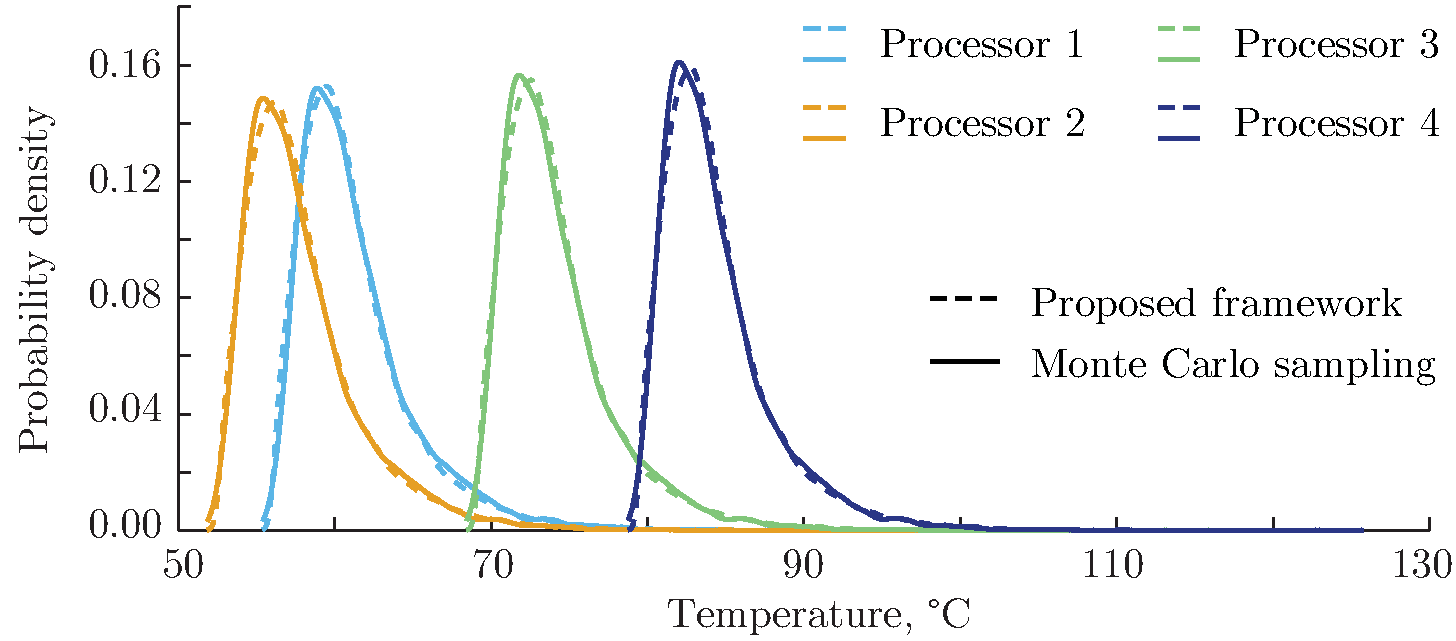
\includegraphics[width=1\linewidth]{include/assets/experimental-results-pdf.pdf}
  \vspace{-2.0em}
  \caption{Probability density functions computed at time 50$\,\text{ms}$ using the proposed framework (the dashed lines) and MC sampling (the solid lines).}
  \flabel{experimental-results-pdf}
\end{figure}

A comparison for a quad-core architecture with a dynamic power profile of $\nsteps = 10^2$ steps is given in \tref{accuracy-eta-0}, \tref{accuracy-eta-0-5}, and \tref{accuracy-eta-1}, which correspond to $\eta = 0$, $\eta = 0.5$, and $\eta = 1$, respectively.
Each table contains three subtables: one for $\eExp$ (the left most), one for $\eVar$ (in the middle), and one for $\ePDF$ (the right most), which is nine subtables in total.
The columns of the tables that corresponding to high values of $\nsamples$ can be used to assess the accuracy of PC expansions; likewise, the rows that correspond to high values of $\pcorder$ can be used to judge about the sufficiency of the MC samples.
One can immediately note that, in all nine subtables, all error metrics tend to decrease from the top left corners (low values of $\pcorder$ and $\nsamples$) to the bottom right corners (high values of $\pcorder$ and $\nsamples$), which suggests that the PC and MC methods converge.

Let us now focus on the PC-based technique.
It can be seen that the deviation of expectation of our approach is small even for $\pcorder = 1$; more precisely, it is bounded by 1\% (see $\eExp$ for $\pcorder \geq 1$ and $\nsamples \geq 10^3$).
The \nrmse\ of variance, $\eVar$, starts from about 90\% for the first-order PC expansions and drops significantly to less than 6\% for the fourth order (see $\eVar$ for $\pcorder \geq 4$ and $\nsamples = 10^5$).
The results of the third error metric, $\ePDF$, allows us to conclude that the \pdfs\ computed by the third-order (and higher) PC expansions closely follow those estimated by the MC technique with large numbers of samples, namely, the observed errors of the proposed framework are bounded by 2\% (see $\ePDF$ for $\pcorder \geq 3$ and $\nsamples \geq 10^4$).
\fref{experimental-results-pdf} gives an example of the \pdf\ obtained using our framework with $\pcorder = 4$ (the dashed lines) along with those estimated by the MC approach with $\nsamples = 10^4$ (the solid lines).
It can be seen that the empirical \pdfs\ tightly match each other.

\begin{table}[b]
  \vspace{-16pt}
  \centering
  \caption{Scaling with the number of processing elements $\cores$.}
  \begin{tabular*}{0.85\linewidth}{p{20pt}crrr}
    \toprule
    $\cores$ & $\vars$ & PC, seconds & MC, hours & Speedup, times \\
    \midrule
    $ 2$ & $2$ & $ 0.32$ & $31.24$ & $3.55 \times 10^5$ \\
    $ 4$ & $3$ & $ 0.45$ & $30.88$ & $2.46 \times 10^5$ \\
    $ 8$ & $4$ & $ 1.26$ & $31.44$ & $9.01 \times 10^4$ \\
    $16$ & $5$ & $ 6.55$ & $38.34$ & $2.11 \times 10^4$ \\
    $32$ & $6$ & $40.29$ & $41.58$ & $3.72 \times 10^3$ \\
    \bottomrule
  \end{tabular*}
  \tlabel{scaling-cores}
  \vspace{5pt}
  \caption{Scaling with the number of steps $\steps$.}
  \begin{tabular*}{0.85\linewidth}{p{42pt}rrr}
    \toprule
    $\steps$ & PC, seconds & MC, hours & Speedup, times \\
    \midrule
    $   10$ & $ 0.04$ & $   0.88$ & $8.19 \times 10^4$ \\
    $ 10^2$ & $ 0.06$ & $   3.12$ & $1.99 \times 10^5$ \\
    $ 10^3$ & $ 0.43$ & $  31.35$ & $2.65 \times 10^5$ \\
    $ 10^4$ & $ 4.35$ & $ 318.00$ & $2.63 \times 10^5$ \\
    $ 10^5$ & $42.23$ & $3110.29$ & $2.65 \times 10^5$ \\
    \bottomrule
  \end{tabular*}
  \tlabel{scaling-steps}
\end{table}

Now we shall take a closer look at the convergence of the MC-based technique. With this in mind, let us concentrate on the rows of \tref{accuracy} that correspond to the PC expansions of high orders.
It can be seen that the MC approach with $\nsamples = 10^2$ has a significantly high error rate, namely, it is above 50\% for variance and above 8\% for \pdfs\ (see $\eVar$ and $\ePDF$ for $\pcorder \geq 3$ and $\nsamples = 10^2$).
The results of MC sampling with $\nsamples = 10^3$ are reasonably more accurate; however, the error of variance is still rather high (see $\eVar$ for $\pcorder = 7$ and $\nsamples = 10^3$).
It should also be noted that, for a fixed $\pcorder \geq 3$, $\eVar$ exhibits a firm decrease even for the transition from $\nsamples = 10^4$ to $\nsamples = 10^5$ (see $\eVar$ for $\pcorder \geq 4$ and $\nsamples \geq 10^4$).
This observation suggests that the previously mentioned errors of the PC approach are overestimated since the maximal number of MC samples, $\nsamples = 10^5$, is not sufficient to reach the accuracy of our framework.
In particular, the results delivered by the fourth-order PC expansions are expected to be more accurate than the reported bound for $\eVar$ of 6\%.

Finally, we would like comment on the effect of the considered correlation patterns.
Although the number of the independent random variables $\vZ(\o)$ changes when $\eta$ is varied, which we shall see in the forthcoming section, the error metrics $\eExp$ and $\ePDF$ do not seem to favor any of the combinations of the correlation kernels.
However, according to $\eVar$, the case with $\eta = 1$, which corresponds to the squared exponential kernel, stands out to be the least error prone.
